% 
% 
%
\section{METHODOLOGY}

I this section, we implement a solver for the 2-D Poisson Equation using the Hybridized SBP-SAT method. We implement our solver in PETSc 

%In this section, we propose an alternative topology, ×Grid, which simplifies client handoff procedures using pyephem’s kelperian orbit models [19], overcoming the limitations of the +Grid described above. Additionally, we describe a low- cost routing scheme atop ×Grid which selects the correct return node without computing the state of the network.

%%%%%%%%%%%%%%%%%%%%%%%%%%%%%%%%%%%%%%%%%%%%%%%%%%%%%%%%%%%%%%%%%%%%%%%%%%
%%%%%%%%%%%%%%%%%%%%%%%%%%%%%%%%%%%%%%%%%%%%%%%%%%%%%%%%%
%%%%%%%%%%%%%%%%%%%%%%%%%%%%%%%%%%%%%%%%%%%%%%%%%%%%%%%%%%%%%%%%%%%%%%%%%%

What is currently lacking in our understanding of the hyrbidized FD and 
FE methods is the relationship between meshing and computational performance. Several authors have discussed numerical performance as it relates to meshing and
the order of the approximation of the PDE being solved \citep{}. However, the discussion of computation performance as it relates to meshing characteristics is limited. This may be in a large part due to the reality that methods that allow the local problems to be solves independent of global trace problem are relatively 
uncommon and specialized. 

There definitionally exists is a relationship between the size of scale of computation and it's performance, but this is less obvious as it relates
to the specifics of the mesh created for a problem. This provokes two 
research questions:

\begin{enumerate}[label=\textbf{\footnotesize RQ\arabic*.}]
	\item {Do we achieve strong-scaling with the hybrid \mbox{SBP-SAT} 
		   method by adding more elements?}
	\item {Is there an ideal number of elements for performance, and does it 
		   vary with other quantities like problem size or thread count?}
\end{enumerate}

%%%%%%%%%%%%%%%%%%%%%%%%%%%%%%%%%%%%%%%%%%%%%%%%%%%%%%%%%%%%%%%%%%%%%%%%%%
\subsection{Problem description} %%%%%%%%%%%%%%%%%%%%%%%%%%%%%%%%%%%%%%%%%
%%%%%%%%%%%%%%%%%%%%%%%%%%%%%%%%%%%%%%%%%%%%%%%%%%%%%%%%%%%%%%%%%%%%%%%%%%

Through the use of the hybridized SBP-SAT method, we investigate 
the shared memory, strong-scaling characteristics of the 2D Poisson 
equation assembled with the SBP-SAT method \citep{kozdon2021hybridized}. 
Whereas PDE performance is largely considered in a weak-scaling context,
we study the strong-scaling characteristics by fixing the number of 
volume points, leveraging the hybrid formulation of the SBP-SAT method, 
to solve a varied size and quantity of independent problems.

\noindent 
We assemble a 2D Poisson equation 
\begin{subequations}
\begin{equation}
	\left( \dfrac{\partial^2}{\partial x^2} + \dfrac{\partial^2}{\partial y^2} \right) u(x, y) = f(x, y) 
\end{equation}
\noindent 
defined over the domain
\begin{equation}
	0 \leq x \leq 1,
\end{equation}
\begin{equation}
	0 \leq y \leq 1,
\end{equation}
\noindent
given the boundary conditions
\begin{equation}
	u(0, y) = \text{sin}(y),
\end{equation}
\begin{equation}
	u(1, y) = \text{sin}(\pi + y),
\end{equation}
\begin{equation}
	\dfrac{\partial u(x, 0)}{\partial y} = -\pi \text{cos}(\pi x),
\end{equation}
\begin{equation}
	\dfrac{\partial u(x, 1)}{\partial y} = -\pi \text{cos}(\pi x)
\end{equation}
\noindent 
and source function
\begin{equation}
	f(x, y) = -2 \pi^2 u(x, y). 
\end{equation}
	\label{eqn:problem_desc}
\end{subequations}
\noindent 
This sets up the manufactured solution
\begin{equation}
	u(x, y) = sin(\pi x + \pi y).
\end{equation}

%%%%%%%%%%%%%%%%%%%%%%%%%%%%%%%%%%%%%%%%%%%%%%%%%%%%%%%%%%%%%%%%%%%%%%%%%%
\subsection{Hybrid scheme} %%%%%%%%%%%%%%%%%%%%%%%%%%%%%%%%%%%%%%%%%%%%%%%
%%%%%%%%%%%%%%%%%%%%%%%%%%%%%%%%%%%%%%%%%%%%%%%%%%%%%%%%%%%%%%%%%%%%%%%%%%

The hybridized SBP-SAT formulation discretizes this problem into the form 
\begin{equation}
    \left[\begin{array}{cc}
        \textbf{M}             & \textbf{F} \\
        \textbf{F}^{\intercal} & \textbf{D}
    \end{array}\right] 
    \left(\begin{array}{c}
        \textbf{u} \\
        \symbf{\lambda}
    \end{array}\right) = 
    \left(\begin{array}{l}
        \bar{\textbf{g}} \\
        \gbd
    \end{array}\right),
    \label{eqn:hybrid_system}
\end{equation}

\noindent
and following from {\color{red} [cite]} we use the Schur complement, $
(\textbf{D} - \textbf{F}^{\intercal} \textbf{M}^{-1} \textbf{F}) 
\symbf{\lambda} = \gbd - \textbf{F}^{\intercal} \textbf{M}^{-1} 
\bar{\textbf{g}}$, to solve this system in two parts: the global problem,

\begin{subequations}
\begin{equation}
\symbf{\lambda}_{\textbf{A}} \coloneqq \gbd - \textbf{F}^{\intercal} \text{solve}(\textbf{M}, \bar{\textbf{g}})
\label{eqn:global_system_a}
\end{equation}
\begin{equation}
\symbf{\lambda}_{\textbf{b}} \coloneqq \textbf{D} - \textbf{F}^{\intercal} \text{solve}(\textbf{M}, \textbf{F})
\label{eqn:global_system_b}
\end{equation}
\begin{equation}
\symbf{\lambda} \coloneqq \text{solve}(\symbf{\lambda}_{\textbf{A}}, \symbf{\lambda}_{\textbf{b}}),
\label{eqn:global_system_c}
\end{equation}
\end{subequations}
\noindent
and the local problem,
\begin{equation} 
\textbf{u} \coloneqq \text{solve}(\textbf{M}, (\bar{\textbf{g}} - \textbf{F} \times \symbf{\lambda})).
\label{eqn:local_system}
\end{equation}

\noindent
In this scheme, multiple elements with continuous domains can be coupled 
with boundary coefficients, similar to fluxes found in finite element 
methods. The boundary coefficients are factored out to $\textbf{F}$ and 
$\textbf{F}^{\intercal}$, leaving $\textbf{M}$ with a block diagonal 
non-zero pattern. 

\begin{aside}
	In this work we consider a specialization of the problem where the 
	number of elements, $\ell^2$, is the square of the number of elements
	on either side of the \emph{global} domain, $\ell$. Additionally, 
	each the number of volume points in each element, $n^2$, is the 
	square of the number of volume points along any side $n$. Finally, 
	there are only 4 interfaces, 1 for each orthogonal face of an element.
\end{aside}

\begin{figure}
	\centering
	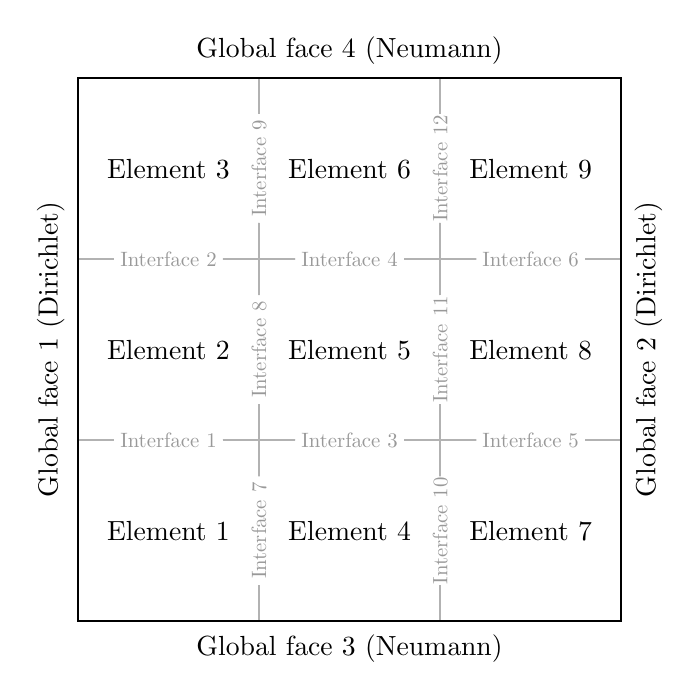
\begin{tikzpicture}[scale=2.3]
\draw[step=1cm,black!30,line width=0.3mm] (0, 0) grid (3, 3);
\draw[line width=0.3mm] (0, 0) rectangle (3, 3);

\fill[white] (0.5cm, 1cm) circle (0.3cm);
\node[color=black!40, scale=0.75] at (0.5cm, 1cm) {Interface 1};
\fill[white] (0.5cm, 2cm) circle (0.3cm);
\node[color=black!40, scale=0.75] at (0.5cm, 2cm) {Interface 2};
\fill[white] (1.5cm, 1cm) circle (0.3cm);
\node[color=black!40, scale=0.75] at (1.5cm, 1cm) {Interface 3};
\fill[white] (1.5cm, 2cm) circle (0.3cm);
\node[color=black!40, scale=0.75] at (1.5cm, 2cm) {Interface 4};
\fill[white] (2.5cm, 1cm) circle (0.3cm);
\node[color=black!40, scale=0.75] at (2.5cm, 1cm) {Interface 5};
\fill[white] (2.5cm, 2cm) circle (0.3cm);
\node[color=black!40, scale=0.75] at (2.5cm, 2cm) {Interface 6};

\fill[white](1cm, 0.5cm) circle (0.3cm);
\node[color=black!40, rotate=90, scale=0.75] at (1cm, 0.5cm) {Interface 7};
\fill[white] (1cm, 1.5cm) circle (0.3cm);
\node[color=black!40, rotate=90, scale=0.75] at (1cm, 1.5cm) {Interface 8};
\fill[white] (1cm, 2.5cm) circle (0.3cm);
\node[color=black!40, rotate=90, scale=0.75] at (1cm, 2.5cm) {Interface 9};
\fill[white] (2cm, 0.5cm) circle (0.3cm);
\node[color=black!40, rotate=90, scale=0.75] at (2cm, 0.5cm) {Interface 10};
\fill[white] (2cm, 1.5cm) circle (0.3cm);
\node[color=black!40, rotate=90, scale=0.75] at(2cm, 1.5cm) {Interface 11};
\fill[white] (2cm, 2.5cm) circle (0.3cm);
\node[color=black!40, rotate=90, scale=0.75] at (2cm, 2.5cm) {Interface 12};


\draw (0.5cm, 0.5cm) -- (0.5cm, 0.5cm) node[anchor=center] {Element 1};
\draw (0.5cm, 1.5cm) -- (0.5cm, 1.5cm) node[anchor=center] {Element 2};
\draw (0.5cm, 2.5cm) -- (0.5cm, 2.5cm) node[anchor=center] {Element 3};
\draw (1.5cm, 0.5cm) -- (1.5cm, 0.5cm) node[anchor=center] {Element 4};
\draw (1.5cm, 1.5cm) -- (1.5cm, 1.5cm) node[anchor=center] {Element 5};
\draw (1.5cm, 2.5cm) -- (1.5cm, 2.5cm) node[anchor=center] {Element 6};
\draw (2.5cm, 0.5cm) -- (2.5cm, 0.5cm) node[anchor=center] {Element 7};
\draw (2.5cm, 1.5cm) -- (2.5cm, 1.5cm) node[anchor=center] {Element 8};
\draw (2.5cm, 2.5cm) -- (2.5cm, 2.5cm) node[anchor=center] {Element 9};


\node[rotate=90] at (-0.15cm, 1.5cm) {Global face 1 (Dirichlet)};
\node[rotate=90] at (3.15cm, 1.5cm) {Global face 2 (Dirichlet)};
\node at (1.5cm, -0.15cm) {Global face 3 (Neumann)};
\node at (1.5cm, 3.15cm)  {Global face 4 (Neumann)};
\end{tikzpicture}
	\caption{An illustration the volume, and arrangement of interfaces 
		described by a 3-by-3 instance of the hybrid problem specified 
		in \eqref{eqn:hybrid_system}.}
	\label{fig:volume_diagram}
\end{figure}

\noindent
This permits us to \textbf{a)} compute much larger problems with less 
memory, especially if the problem is largely homogeneous, and \textbf{b)} 
reduce the computational complexity of solving the system by instead 
solving several smaller systems. In both cases this allows us express the 
equations (\ref{eqn:global_system_a}--\ref{eqn:global_system_c}, 
\ref{eqn:local_system}) as a concatenation of smaller problems. 

To form the smaller problems we decompose the sub-matrices 
$\textbf{M}$, $\textbf{F}$, $\textbf{F}^{\intercal}$, and $\textbf{D}$. 
For example, as $\textbf{M}$ is block-diagonal, we store each non-zero 
block of $\textbf{M}$ as distinct matrices. A similar structure exists 
for $\textbf{F}$ and $\textbf{F}^{\intercal}$. 

In a 3-by-3 example of the problem we reconstruct $\textbf{F}$ from the 
representational matrix, $\textbf{F}^{\text{ind}}$, and the set of unique
$\textbf{F}^{i}$ sub-matrices, substituting the appropriate sub-matrix in
place of the integer value, \emph{i.e.},
\begin{subequations}
\begin{equation}
	\textbf{F} = \textbf{F}^{\text{ind}}\left[\textbf{F}^{i}/i\right] \text{ where } i \neq 0,
\end{equation}
\begin{equation}
	{\footnotesize
    \begin{array}{c}
        {\color{gray} \hspace{-1em} \textit{Interface index}} \\
        {\color{gray}
        \begin{array}{C{0.25em}C{0.5em}C{0.5em}C{0.5em}C{0.5em}C{0.5em}C{0.5em}C{0.5em}C{0.5em}C{0.5em}C{0.5em}C{0.5em}C{0.5em}C{0.5em}}
        {}&{1}&{2}&{3}&{4}&{5}&{6}&{7}&{8}&{9}&{10}&{11}&{12}&{}\\
        \end{array}} \\
        \textbf{F}^{\text{ind}} = \left[\begin{array}{cccccccccccc}
         4 &{·}&{·}&{·}&{·}&{·}& 2 &{·}&{·}&{·}&{·}&{·}\\
         3 & 4 &{·}&{·}&{·}&{·}&{·}& 1 &{·}&{·}&{·}&{·}\\
        {·}& 3 &{·}&{·}&{·}&{·}&{·}&{·}& 2 &{·}&{·}&{·}\\
        {·}&{·}& 4 &{·}&{·}&{·}& 1 &{·}&{·}& 2 &{·}&{·}\\
        {·}&{·}& 3 & 4 &{·}&{·}&{·}& 1 &{·}&{·}& 2 &{·}\\
        {·}&{·}&{·}& 3 &{·}&{·}&{·}&{·}& 1 &{·}&{·}& 2 \\
        {·}&{·}&{·}&{·}& 4 &{·}&{·}&{·}&{·}& 1 &{·}&{·}\\
        {·}&{·}&{·}&{·}& 3 & 4 &{·}&{·}&{·}&{·}& 1 &{·}\\
        {·}&{·}&{·}&{·}&{·}& 3 &{·}&{·}&{·}&{·}&{·}& 1 \\
        
        \end{array}\right] {\color{gray}
        \begin{array}{C{1em}}
        1 \\ 2 \\ 3 \\ 4 \\ 5 \\ 6 \\ 7 \\ 8 \\ 9
        \end{array}{\rotatebox[origin=c]{90}{\textit{Block index}}}} \\
    \end{array}}
\end{equation}
\begin{equation}
	\left\{\textbf{F}^{1},\textbf{F}^{2},\textbf{F}^{3},\textbf{F}^{4}
	\right\}.
\end{equation}
\end{subequations}

\noindent
With these decomposed matrices, we compute several sub-sections of each computation and with a lower memory footprint. This decomposition strategy
is a known characteristic of hyrbidized methods, and is the fundamental 
reason to utilize these methods, in particular for larger problems sizes
within a shared-memory context \citep{kozdon2021hybridized, 
kolev2021efficient, fernandez2017hybridized}. 

\begin{figure}
	\centering
	
\begin{tikzpicture}[scale=1.6]
\filldraw[color=black!10] (0, 0) rectangle (3, 3);
\filldraw[color=black!30, text=black] (0.00cm, 2.66cm) rectangle (0.33cm, 3.00cm) node[pos=.5] {$\textbf{M}_1$};
\filldraw[color=black!30, text=black] (0.33cm, 2.33cm) rectangle (0.66cm, 2.66cm) node[pos=.5] {$\textbf{M}_2$};
\filldraw[color=black!30, text=black] (0.66cm, 2.00cm) rectangle (1.00cm, 2.33cm) node[pos=.5] {$\textbf{M}_3$};
\filldraw[color=black!30, text=black] (1.00cm, 1.66cm) rectangle (1.33cm, 2.00cm) node[pos=.5] {$\textbf{M}_4$};
\filldraw[color=black!30, text=black] (1.33cm, 1.33cm) rectangle (1.66cm, 1.66cm) node[pos=.5] {$\textbf{M}_5$};
\filldraw[color=black!30, text=black] (1.66cm, 1.00cm) rectangle (2.00cm, 1.33cm) node[pos=.5] {$\textbf{M}_6$};
\filldraw[color=black!30, text=black] (2.00cm, 0.66cm) rectangle (2.33cm, 1.00cm) node[pos=.5] {$\textbf{M}_7$};
\filldraw[color=black!30, text=black] (2.33cm, 0.33cm) rectangle (2.66cm, 0.66cm) node[pos=.5] {$\textbf{M}_8$};
\filldraw[color=black!30, text=black] (2.66cm, 0.00cm) rectangle (3.00cm, 0.33cm) node[pos=.5] {$\textbf{M}_9$};

\filldraw[color=black!10,xshift=0.1cm] (3, 0) rectangle (4.33, 3);

\filldraw[color=red!30,xshift=0.1cm] (3.00cm, 2.66cm) rectangle (3.11cm, 3.00cm);
\filldraw[color=red!30,xshift=0.1cm] (3.11cm, 2.33cm) rectangle (3.22cm, 2.66cm);
\filldraw[color=red!30,xshift=0.1cm] (3.22cm, 1.66cm) rectangle (3.33cm, 2.00cm);
\filldraw[color=red!30,xshift=0.1cm] (3.33cm, 1.33cm) rectangle (3.44cm, 1.66cm);
\filldraw[color=red!30,xshift=0.1cm] (3.44cm, 0.66cm) rectangle (3.55cm, 1.00cm);
\filldraw[color=red!30,xshift=0.1cm] (3.55cm, 0.33cm) rectangle (3.66cm, 0.66cm);

\filldraw[color=green!30,xshift=0.1cm] (3.00cm, 2.33cm) rectangle (3.11cm, 2.66cm);
\filldraw[color=green!30,xshift=0.1cm] (3.11cm, 2.00cm) rectangle (3.22cm, 2.33cm);
\filldraw[color=green!30,xshift=0.1cm] (3.22cm, 1.33cm) rectangle (3.33cm, 1.66cm);
\filldraw[color=green!30,xshift=0.1cm] (3.33cm, 1.00cm) rectangle (3.44cm, 1.33cm);
\filldraw[color=green!30,xshift=0.1cm] (3.44cm, 0.33cm) rectangle (3.55cm, 0.66cm);
\filldraw[color=green!30,xshift=0.1cm] (3.55cm, 0.00cm) rectangle (3.66cm, 0.33cm);

\filldraw[color=violet!30,xshift=0.1cm] (3.66cm, 2.66cm) rectangle (3.77cm, 3.00cm);
\filldraw[color=violet!30,xshift=0.1cm] (3.77cm, 2.33cm) rectangle (3.88cm, 2.66cm);
\filldraw[color=violet!30,xshift=0.1cm] (3.88cm, 2.00cm) rectangle (4.00cm, 2.33cm);
\filldraw[color=violet!30,xshift=0.1cm] (4.00cm, 1.66cm) rectangle (4.11cm, 2.00cm);
\filldraw[color=violet!30,xshift=0.1cm] (4.11cm, 1.33cm) rectangle (4.22cm, 1.66cm);
\filldraw[color=violet!30,xshift=0.1cm] (4.22cm, 1.00cm) rectangle (4.33cm, 1.33cm);

\filldraw[color=orange!30,xshift=0.1cm] (3.66cm, 1.66cm) rectangle (3.77cm, 2.00cm);
\filldraw[color=orange!30,xshift=0.1cm] (3.77cm, 1.33cm) rectangle (3.88cm, 1.66cm);
\filldraw[color=orange!30,xshift=0.1cm] (3.88cm, 1.00cm) rectangle (4.00cm, 1.33cm);
\filldraw[color=orange!30,xshift=0.1cm] (4.00cm, 0.66cm) rectangle (4.11cm, 1.00cm);
\filldraw[color=orange!30,xshift=0.1cm] (4.11cm, 0.33cm) rectangle (4.22cm, 0.66cm);
\filldraw[color=orange!30,xshift=0.1cm] (4.22cm, 0.00cm) rectangle (4.33cm, 0.33cm);

\filldraw[color=black!10,yshift=-0.1cm] (0, -1.33) rectangle (3, 0);

\begin{scope}[rotate around={-90:(0,0)},yscale=1,xscale=-1,xshift=-3.86cm,yshift=-0.33cm]
 
\filldraw[color=red!30,xshift=0.1cm] (3.00cm, 2.66cm) rectangle (3.11cm, 3.00cm);
\filldraw[color=red!30,xshift=0.1cm] (3.11cm, 2.33cm) rectangle (3.22cm, 2.66cm);
\filldraw[color=red!30,xshift=0.1cm] (3.22cm, 1.66cm) rectangle (3.33cm, 2.00cm);
\filldraw[color=red!30,xshift=0.1cm] (3.33cm, 1.33cm) rectangle (3.44cm, 1.66cm);
\filldraw[color=red!30,xshift=0.1cm] (3.44cm, 0.66cm) rectangle (3.55cm, 1.00cm);
\filldraw[color=red!30,xshift=0.1cm] (3.55cm, 0.33cm) rectangle (3.66cm, 0.66cm);

\end{scope}
\begin{scope}[rotate around={-90:(0,0)},yscale=1,xscale=-1,xshift=-3.86cm,yshift=0.34cm]

\filldraw[color=green!30,xshift=0.1cm] (3.00cm, 2.33cm) rectangle (3.11cm, 2.66cm);
\filldraw[color=green!30,xshift=0.1cm] (3.11cm, 2.00cm) rectangle (3.22cm, 2.33cm);
\filldraw[color=green!30,xshift=0.1cm] (3.22cm, 1.33cm) rectangle (3.33cm, 1.66cm);
\filldraw[color=green!30,xshift=0.1cm] (3.33cm, 1.00cm) rectangle (3.44cm, 1.33cm);
\filldraw[color=green!30,xshift=0.1cm] (3.44cm, 0.33cm) rectangle (3.55cm, 0.66cm);
\filldraw[color=green!30,xshift=0.1cm] (3.55cm, 0.00cm) rectangle (3.66cm, 0.33cm);

\end{scope}
\begin{scope}[rotate around={-90:(0,0)},yscale=1,xscale=-1,xshift=-5.19cm,yshift=1cm] 

\filldraw[color=orange!30,xshift=0.1cm] (3.66cm, 1.66cm) rectangle (3.77cm, 2.00cm);
\filldraw[color=orange!30,xshift=0.1cm] (3.77cm, 1.33cm) rectangle (3.88cm, 1.66cm);
\filldraw[color=orange!30,xshift=0.1cm] (3.88cm, 1.00cm) rectangle (4.00cm, 1.33cm);
\filldraw[color=orange!30,xshift=0.1cm] (4.00cm, 0.66cm) rectangle (4.11cm, 1.00cm);
\filldraw[color=orange!30,xshift=0.1cm] (4.11cm, 0.33cm) rectangle (4.22cm, 0.66cm);
\filldraw[color=orange!30,xshift=0.1cm] (4.22cm, 0.00cm) rectangle (4.33cm, 0.33cm);

\end{scope}

\begin{scope}[rotate around={-90:(0,0)},yscale=1,xscale=-1,xshift=-5.19cm,yshift=-1cm]

\filldraw[color=violet!30,xshift=0.1cm] (3.66cm, 2.66cm) rectangle (3.77cm, 3.00cm);
\filldraw[color=violet!30,xshift=0.1cm] (3.77cm, 2.33cm) rectangle (3.88cm, 2.66cm);
\filldraw[color=violet!30,xshift=0.1cm] (3.88cm, 2.00cm) rectangle (4.00cm, 2.33cm);
\filldraw[color=violet!30,xshift=0.1cm] (4.00cm, 1.66cm) rectangle (4.11cm, 2.00cm);
\filldraw[color=violet!30,xshift=0.1cm] (4.11cm, 1.33cm) rectangle (4.22cm, 1.66cm);
\filldraw[color=violet!30,xshift=0.1cm] (4.22cm, 1.00cm) rectangle (4.33cm, 1.33cm);

\end{scope}

\filldraw[color=black!10,xshift=0.1cm,yshift=-0.1cm] (3, -1.33) rectangle (4.33, 0);

\draw[color=black!30,xshift=0.1cm,yshift=-0.1cm] (3, 0) -- (4.33, -1.33);

\draw [black, thick] (-0.1,-1.43) to [square left brace] (-0.1,3);

\draw [black, thick] (4.53,-1.43) to [square right brace] (4.53,3);

\filldraw[draw=black,fill=white] (0.39cm, -2.1cm) rectangle (4.09cm, -1.53cm);

\filldraw[color=black!10,xshift=0.49cm, text=black] (0cm, -2cm) rectangle (0.5cm, -1.63cm) node[pos=.5] {$0$};
\filldraw[color=black!30,xshift=1.09cm, text=black] (0cm, -2cm) rectangle (0.5cm, -1.63cm) node[pos=.5] {$\textbf{M}_i$};
\filldraw[color=red!30,xshift=1.69cm, text=black] (0cm, -2cm) rectangle (0.5cm, -1.63cm) node[pos=.5] {$\textbf{F}^1$};
\filldraw[color=green!30,xshift=2.29cm, text=black] (0cm, -2cm) rectangle (0.5cm, -1.63cm) node[pos=.5] {$\textbf{F}^2$};
\filldraw[color=violet!30,xshift=2.89cm, text=black] (0cm, -2cm) rectangle (0.5cm, -1.63cm) node[pos=.5] {$\textbf{F}^3$};
\filldraw[color=orange!30,xshift=3.49cm, text=black] (0cm, -2cm) rectangle (0.5cm, -1.63cm) node[pos=.5] {$\textbf{F}^4$};
%\draw [decorate,decoration={brace,amplitude=10pt},xshift=-2pt,yshift=0pt]
%(0cm,2cm) -- (0cm,3cm) node [black,midway,xshift=-0.6cm] 
%{\footnotesize $n$};

\end{tikzpicture}

	\caption{A visualization of the non-zero pattern of the matrix 
	operator of a 3-by-3 instance of the hybrid problem specified 
	in eq. \eqref{eqn:hybrid_system}.}
	\label{fig:block_diagram}
\end{figure}

%%%%%%%%%%%%%%%%%%%%%%%%%%%%%%%%%%%%%%%%%%%%%%%%%%%%%%%%%%%%%%%%%%%%%%%%%%
\subsection{Complexity of the trace system} %%%%%%%%%%%%%%%%%%%%%%%%%%%%%%
%%%%%%%%%%%%%%%%%%%%%%%%%%%%%%%%%%%%%%%%%%%%%%%%%%%%%%%%%%%%%%%%%%%%%%%%%%


The hybrid formulation permits us to compute much larger problems with 
less memory and fewer reads, especially if the problem is mostly 
homogeneous. This is of particular interest as the 3 significant 
computations used in computing this problem \emph{i.e.}, MatMult, SpMV, 
and linear solve, are memory-bound operations. Additionally, we 
reduce the computational complexity of solving the system by instead 
solving several smaller systems. In both cases this allows us to express 
the equations (\ref{eqn:global_system_a}--\ref{eqn:global_system_c}, 
\ref{eqn:local_system}) as a concatenation of decomposed, smaller problems.

To evaluate this the performance characteristics we fix the global number 
of volume points, $\bar{n}^2$, and vary the number of elements, to 
understand if there exists an optimal trade-off between the size of the 
decomposed matrices and quantity of computations derived from the 
decomposed matrices.

%%%%%%%%%%%%%%%%%%%%%%%%%%%%%%%%%%%%%%%%%%%%%%%%%%%%%%%%%%%%%%%%%%%%%%%%%%
\subsubsection{Computing the trace inverse product} %%%%%%%%%%%%%%%%%%%
%%%%%%%%%%%%%%%%%%%%%%%%%%%%%%%%%%%%%%%%%%%%%%%%%%%%%%%%%%%%%%%%%%%%%%%%%%

\noindent
In our PETSc-based C++ implementation, the product 
$\textbf{M}^{-1}\textbf{F}$ is computed from a series a series of solves 

we store $\textbf{F}$ as a vector 
of vectors to compute $\textbf{M}^{-1}\textbf{F}$. That is, for each 
directional $\textbf{F}^k$ boundary we store a list of $n$ vectors

\begin{equation}
	\textbf{F}^k = \left[\textbf{f}^k_1 \cdots \textbf{f}^k_n\right] 
	\in \mathbb{R}^{n \times n^2}.
\end{equation} 

\noindent
Here, each vector $\textbf{f}^k_i$ is implemented as a PetscVector object.
This method is in contrast to storing $\textbf{F}$ contiguously, and 
allows for the computation of $\textbf{M}^{-1}\textbf{F}$ from the local 
matrices of $\textbf{M}$, stored similarly as

\begin{equation}
	\textbf{M} = \left\{\textbf{M}_1 \cdots \textbf{M}_p\right\} \in 
	\mathbb{R}^{\ell^2 n^2 \times \ell^2 n^2}, p \leq \ell^2.
\end{equation} 

\noindent 
Where $p$ denotes the number of unique local matrix operators in 
$\textbf{M}$. 

With this we compute the intermediate result $\textbf{M}^{-1}\textbf{F}$, 
performing a linear solve of every unique local matrix operator, and 
every vector of every directional boundary coefficient matrix 

\begin{equation}
	\text{solve}(\textbf{M}_{i}, \textbf{F}^{k}_j) \text{  for }
	\begin{array}{l}
		0 < i \leq p, \\
		0 < j \leq n, \\
		0 < k \leq 4. \\ 
	\end{array}
	\label{eqn:mfsolves}
\end{equation}

\noindent
This result has a similar non-zero pattern as $\textbf{F}$, following the same symbolic block structure. In our implementation we solve this system through direct solvers made available through PETSc. 

\begin{aside}
	In the homogeneous Poisson equation in Eq. \eqnref{eqn:problem_desc} we have 
	\begin{equation}
		p = \begin{cases}
		    \ell &  0 \leq \ell < 3 \\ 
			3 &  3 \leq \ell \\ 
		\end{cases}.
	\end{equation} 
	\noindent 
	When $p = 3$ we have one unique $\textbf{M}_i$ for the elements along the top Neumann boundaries, the bottom Neumann boundaries, and the interior elements. 
	Since $p$ is constant when $\ell \geq 3$, increasing the number of elements, $\ell^2$ decreases the number of solves in \eqnref{eqn:mfsolves}, as well as the size of each solve, for a constant global volume, $\bar{n}^2$. 
\end{aside}

For a fixed $\bar{n}^2$ we write the number of 

%
%
%
\subsubsection{Computing the trace MatMult} 

%
%
%
The non-zero structure of the matrix used to solve $\symbf{\lambda}$, \emph{i.e.}, \eqnref{eqn:global_system_a} provides insight into the complexity the two operations in $\textbf{F}^{\intercal} \times \textbf{M}^{-1} \textbf{F}$. 
The memory needed to store the decomposed matrix consisting of $\textbf{M}$, $\textbf{F}$, $\textbf{F}^{\intercal}$, $\textbf{D}$ is minimally the size of each unique, decomposed sub-matrix. 
This is illustrated in \figref{fig:block_diagram}, as the $\textbf{F}$ and $\textbf{F}^{\intercal}$ matrices only contain 4 unique sub-matrices, $\textbf{F}^{1}$, $\textbf{F}^{2}$, $\textbf{F}^{3}$, and $\textbf{F}^{4}$. 
The uniqueness of $\textbf{M}$ is less obvious here, but by \figref{fig:volume_diagram} we see that there are only 3 unique local problems, one with a Neumann boundary on face 4, another with a Neumann boundary on face 3, and a final problem with a no Neumann boundary conditions.

Fixing the number of global volume points, $\bar{n}^2$, the number of local volume points per row, $n$, is given in terms of the number of elements per row, $n = \bar{n} / \ell$, and similarly the number of interfaces can be written as $r = 2\ell^2 - 2\ell$. 
The dimensions of $\symbf{\lambda}_\textbf{A}$ can then be written as 
\begin{equation}
	\symbf{\lambda}_\textbf{A} \in \mathbb{R}^{rn \times rn} \equiv \mathbb{R}^{2\bar{n}\ell - 2\bar{n} \times 2\bar{n}\ell - 2\bar{n}}. 
\end{equation}
The number of non-zeros in $\textbf{F}^{\intercal}(\textbf{M}^{-1}\textbf{F})$ are given by
\begin{subequations}
\begin{equation}
	n \sum_{i=1}^{\ell^2} (\phi_i^2)
	\label{eqn:nz_sum}
\end{equation}
where
\begin{equation}
	\textbf{F}^{\text{ind}} = \left[\textbf{f}^{\text{ind}}_1 \cdots \textbf{f}^{\text{ind}}_{\ell^2}\right] \in \mathbb{Z}^{\ell^2 \times r},
\end{equation}
\begin{equation}
	\phi = \left[ \text{nnz}(\textbf{f}^{\text{ind}}_1) \cdots \text{nnz}(\textbf{f}^{\text{ind}}_{\ell^2}) \right] \in \mathbb{Z}^{\ell^2}, 
\end{equation}
\end{subequations}
or, the sum of the square of the number of internal interfaces per element. With the additional constraints we have placed on this problem, we can write $\phi$ as 
\begin{equation}
	\phi = \left[ \underbrace{2, 2, 2, 2}_{4}, \underbrace{3 \cdots 3}_{4\ell - 8}, \underbrace{4 \cdots 4}_{(\ell-2)^2} \right] \in \mathbb{Z}^{\ell^2}, 
\end{equation}
where $2\text{'s}$ denote the corner elements, $3\text{'s}$ denote the boundary elements, and $4\text{'s}$ denote the internal elements. In eq. \eqref{eqn:nz_sum} we square each $\phi_i$ because $\textbf{F}^{\intercal}$ and  $\textbf{M}^{-1}\textbf{F}$ can both be derived from substitutions of $\textbf{F}^{\text{ind}}$, and the sum is multiplied by $n$ there are 

The ordering of the rows in $\textbf{F}^{\text{ind}}$ may not be equivalent in this case, but the final sum will be identical. Throughout the rest of the problem this is not an issue if the ordering remains consistent. 

With this, we derive the non-zero density of $\textbf{F}^{\intercal}\textbf{M}^{-1}\textbf{F}$ as a function of the number of elements per row 
\begin{equation}
	\begin{aligned}
	\text{nzd}(\ell) &= \frac{\bar{n}/\ell (16\ell^2 - 28\ell + 8)}{(2\bar{n}\ell - 2\bar{n})^2} \\
	&= \frac{4\ell^2 - 7\ell + 2}{\bar{n}\ell(\ell-1)^2}.
	\end{aligned}
\end{equation}

\begin{figure}
	{\centering
	\begin{subfigure}{\columnwidth}
		\centering
		\pgfplotsset{compat=newest, width=\columnwidth}
\begin{tikzpicture}
\begin{axis}[
  /pgf/number format/1000 sep={\,},
  height=2in,
	xlabel={\small $\ell^2$ (total elements)},
  xtick={9, 144, 484, 1024},
  ymode=log,
  ylabel={\small Non-zero density of $\symbf{\lambda}_{\textbf{A}} \text{(log)}$},
  legend style={
    font=\footnotesize}, 
  legend cell align={left}]
    \addplot[
    	select coords between index={1}{2500},
    	color=red,smooth,thick] 
    	table[col sep=comma,header=false,
      	x index=0,y index=1] {data/density1};
    \addlegendentry{$\bar{n}^2 = 1\text{E+}4$}
    \addplot[
    	select coords between index={1}{2500},
    	color=blue,smooth,thick] table[col sep=comma,header=false,
      x index=0,y index=1] {data/density2};
    \addlegendentry{$\bar{n}^2 = 1\text{E+}5$}
    \addplot[
    	select coords between index={1}{2500},
    	color=black,smooth,thick] table[col sep=comma,header=false,
      	x index=0,y index=1] {data/density3};
    \addlegendentry{$\bar{n}^2 = 1\text{E+}6$}
\end{axis}
\end{tikzpicture}
	\end{subfigure}
	\begin{subfigure}{\columnwidth}
		\centering
		\pgfplotsset{compat=newest, width=\columnwidth}
\begin{tikzpicture}
\begin{axis}[height=2in,
	xlabel={$\ell^2$ (total elements)},
  xtick={9, 144, 484, 1024},
    ylabel={Non-zeros in $\symbf{\lambda}_{\textbf{A}}$},
    legend style={font=\footnotesize},
    legend cell align={left}]
    \addplot[
    	select coords between index={1}{2500},
    	color=red,smooth,thick] 
    	table[col sep=comma,header=false,
      	x index=0,y index=1] {data/nonzeros1};
    \addlegendentry{$\bar{n}^2 = 10000$}
    \addplot[
    	select coords between index={1}{2500},
    	color=blue,smooth,thick] table[col sep=comma,header=false,
      x index=0,y index=1] {data/nonzeros2};
    \addlegendentry{$\bar{n}^2 = 100000$}
    \addplot[
    	select coords between index={1}{2500},
    	color=black,smooth,thick] table[col sep=comma,header=false,
      	x index=0,y index=1] {data/nonzeros3};
    \addlegendentry{$\bar{n}^2 = 1000000$}
\end{axis}
\end{tikzpicture}
	\end{subfigure}}
	\caption[The non-zero density of $\symbf{\lambda}_{\textbf{A}}$ 
	plotted as a function of the total number of elements.]{\textbf{The non-zero 
	density of $\symbf{\lambda}_{\textbf{A}}$ plotted as a function of 
	the total number of elements.} Though increasing the number of elements adds non-zeros for every new 
	interface between two elements, the size of the matrix increases 
	proportionally faster.}
	\label{fig:nz_density} 
\end{figure}

\noindent
This is plotted in fig. \ref{fig:nz_density} for several values of $\bar{n}$ alongside of a plot of the quantity of non-zeros. Here we see that when the $\bar{n}^2$ is fixed, the size of the trace system is governed by a 3rd degree polynomial while the quantity of non-zeros is 2nd order, resulting in different non-zero densities depending on the $\ell$. This is significant as performance often depends on the choice of solvers and preconditioners and that are well suited to the size of non-zero pattern of the problem \citep{bollhofer2020state}. % todo: find more sources here 

In our implementation each non-zero corresponds to a vector dot product between a a non-zero row of the sub-matrices of $\textbf{F}^{\intercal}$ and a decomposed result of computing  $\textbf{M}^{-1}\textbf{F}$

\noindent
We store $\textbf{F}$ as a vector of vectors to compute $\textbf{M}^{-1}\textbf{F}$. That is, for each directional $\textbf{F}^k$ boundary we store a list of $N$ vectors

\begin{equation}
	\textbf{F}^k = \left[\textbf{f}^k_1 \cdots \textbf{f}^k_N\right] \in \mathbb{R}^{N \times N^2}.
\end{equation} 

\noindent
In our implementation each vector $\textbf{f}^k_i$ is a PETSc vector. This method is in contrast to storing $\textbf{F}$ contiguously, and allows for the computation of $\textbf{M}^{-1}\textbf{F}$ from the local matrices of $\textbf{M}$, stored similarly as

\begin{equation}
	\textbf{M} = \left\{\textbf{M}_1 \cdots \textbf{M}_p\right\} \in \mathbb{R}^{N_{E}N^2 \times N_{E}N^2}, p \leq E.
\end{equation} 

\noindent 
Where $p$ denotes the number of unique local matrix operators in $\textbf{M}$. 

With this we compute the intermediate result $\textbf{M}^{-1}\textbf{F}$, performing a linear solve of every unique local matrix operator, and every vector of every directional boundary coefficient matrix 

\begin{equation}
	\text{solve}(\textbf{M}_{i}, \textbf{F}^{k}_j) \text{  for }
	\begin{array}{l}
		0 < i \leq p, \\
		0 < j \leq N, \\
		0 < k \leq D. \\ 
	\end{array}
\end{equation}

\noindent
The resultant has a similar non-zero pattern as $\textbf{F}$, following the same symbolic block structure. In our implementation we solve this system through direct solvers made available through PETSc. 

\begin{aside}
	In the homogeneous Poisson equation we have assembled in 
	eq {\color{red} ?? } 

	\begin{equation}
		p = \begin{cases}
		    N_{EF} &  0 \leq N_{EF} < 3 \\ 
			3 &  3 \leq N_{EF} \\ 
		\end{cases}.
	\end{equation} 

	\noindent 
	When $p = 3$ we have one unique $\textbf{M}_i$ for the elements 
	along the top Neumann boundaries, the bottom Neumann boundaries, 
	and the interior elements. Since $p$ is constant when 
	$E \geq 3$, computational complexity decreases \emph{weakly} 
	as the number of elements in the system increases. Additionally, 
	if we fix $N^2E^2$ and increase $E$, we decrease the size of 
	each solve.
\end{aside}

\noindent
The resultant $\textbf{M}^{-1}\textbf{F}$ is stored as $p \times D \times N$ PETSc vectors of length $N^2$, i.e.,
\begin{subequations}
\begin{equation}
	\textbf{M}^{-1}\textbf{F} = [\alpha_{111} \cdots \alpha_{ijk} \cdots \alpha_{NDp}] \in \mathbb{R}^{pDN \times N^2},
\end{equation}
\begin{equation}
	\alpha_{ijk} = \text{solve}(\textbf{M}_i, \textbf{f}_{j}^{k}).
\end{equation}
 This is used in the matrix product $(\textbf{F}^{\intercal}) \times (\textbf{M}^{-1}\textbf{F})$, computing
\begin{equation}
	\Phi = N \sum_{i = 1}^{E} (\phi_i^2)
\end{equation}
vector dot products s.t.,
\begin{equation}
	\textbf{F}^{\text{ind}} = \left[\textbf{f}^{\text{ind}}_1 \cdots \textbf{f}^{\text{ind}}_{E}\right] \in \mathbb{Z}^{E \times I},
\end{equation}
\begin{equation}
	\phi = \left[ \text{nnz}(\textbf{f}^{\text{ind}}_1) \cdots \text{nnz}(\textbf{f}^{\text{ind}}_E) \right] \in \mathbb{Z}^{E}.
\end{equation}
Thus we have 
\begin{equation}
	(\textbf{F}^{\intercal}) \times (\textbf{M}^{-1}\textbf{F}) = 
	\left[\begin{array}{c}
		\beta_{1 1 1} \cdots \beta_{\phi_1 \phi_1 N} \in \mathbb{R}^{\phi_1^2N} \\ 
		\vdots \\
		\beta_{1 1 1} \cdots \beta_{\phi_E \phi_E N} \in \mathbb{R}^{\phi_E^2N} 
	\end{array}\right] 
\end{equation}
\begin{equation}
	\beta_{i j k l} = \alpha_{iyl} \textbf{f}^{u}_{l}, \text{ where } y = \text{nzval}(\textbf{f}^{\text{ind}}_{ij}), u = \text{nzval}(\textbf{f}^{\text{ind}}_{ik}),
\end{equation}
\end{subequations}
where $\text{nzval}(v_i)$ returns the $i\text{th}$ non-zero value in the vector $v$. Notably here the result is not square of all non-zeros in $\textbf{F}^\text{ind}$, but the sum of the squares of each row in $\textbf{F}^\text{ind}$, making the storage dependent upon $p$, the number unique elements and the sparsity of $\textbf{F}$. 

The index for any scalar value $\beta_{i j k l}$ in the matrix representation of $\textbf{F}^{\intercal}\textbf{M}^{-1}\textbf{F}$ is given as 
\begin{equation}
[(N - 1) i + \text{nzind}(\textbf{f}^{\text{ind}}_{ij}) + l, (N - 1) i + \text{nzind}(\textbf{f}^{\text{ind}}_{ik}) + l]
\end{equation}
\noindent
where $\text{nzind}(v_i)$ returns the index of the $i\text{th}$ non-zero of the vector $v$. Since 
%\begin{}

\subsection{Computational model}
\begin{equation}
\begin{split}
	\text{FLOPs} = & \underbrace{2(\bar{n}/\ell)^2 (16\ell^2 - 28\ell + 8) + 4\ell(
	\bar{n})^3}_{\text{compute }\textbf{F}^{\intercal} \textbf{M}^{-1} \textbf{F}} + \\
	& \underbrace{2 \bar{n}^2 / \ell + \bar{n}^3 / \ell^2}_{\text{compute }\textbf{F}^{\intercal} \textbf{M}^{-1} \bar{g}} 
	+ \underbrace{\bar{n}^3 / \ell^2 }_{\text{solve locals}} 
	+ \underbrace{(2\ell \bar{n} - 2\bar{n})^3}_{\text{solve } \lambda} 
\end{split}
\end{equation}


% \textbf{F}^{\intercal} \textbf{M}^{-1} \textbf{F}

